\section{Perception and Sensing}
\label{sec:perception_sensing}

\subsection{SLAM and Sensor Fusion Implementation}

Accurate localization in dynamic social environments presents unique challenges for autonomous robots, requiring robust pose estimation that maintains accuracy during extended operation while enabling reliable human-robot interaction. The traditional visual odometry approaches suffer from cumulative drift errors that compromise positioning accuracy over time, particularly in feature-poor environments common in indoor social settings.

\subsubsection{RTABMap Visual SLAM Implementation}

To address the fundamental localization requirements, the system integrates RTABMap visual SLAM with the Oak-D Pro stereo camera, providing visual-inertial odometry and mapping capabilities optimized for social robot applications. The implementation leverages the DepthAI ecosystem through the \texttt{depthai\_examples} package for optimized camera drivers and ROS2 integration.

\paragraph{Oak-D Pro Camera Integration}

The Oak-D Pro operates at 400p mono resolution to balance processing performance with image quality on the Orin Nano platform. The \texttt{stereo\_inertial\_node.launch.py} configuration publishes synchronized streams on \texttt{/right/image\_rect}, \texttt{/stereo/depth}, and \texttt{/right/camera\_info}, with depth alignment disabled (\texttt{depth\_aligned: false}) for processing efficiency. Factory calibration data embedded in the Oak-D Pro hardware ensures accurate depth estimation and stereo baseline measurements, while the \texttt{oak-d-base-frame} serves as the primary coordinate reference for consistent transformations.

The four-node RTABMap architecture includes \texttt{rgbd\_sync} for temporal alignment of RGB and depth streams, \texttt{rgbd\_odometry} for continuous pose estimation, the main \texttt{rtabmap} node for loop closure detection and map management, and \texttt{imu\_filter\_madgwick\_node} for quaternion computation from raw IMU data in ENU world frame without magnetic compensation (\texttt{use\_mag: false}).

\paragraph{Dual-Mode Operation}

The system supports both mapping and localization modes through dedicated launch configurations. Mapping mode (\texttt{rtab\_mapping.launch.py}) enables full SLAM functionality with parameters \texttt{subscribe\_rgbd: True}, \texttt{subscribe\_odom\_info: True}, \texttt{approx\_sync: False} for precise temporal alignment, and \texttt{wait\_imu\_to\_init: True} for proper IMU initialization. The mapping process maintains visual landmarks and occupancy grid information in the \texttt{\textasciitilde/rtabmap.db} database for future relocalization.

Localization mode (\texttt{rtab\_localization.launch.py}) loads existing maps with \texttt{localization: True} and \texttt{Mem/IncrementalMemory: False} to prevent map modifications. The \texttt{Rtabmap/DetectionRate: 3.0} parameter optimizes loop closure detection frequency, balancing computational load against relocalization performance for operation in known environments.

\begin{figure}[H]
    \centering
    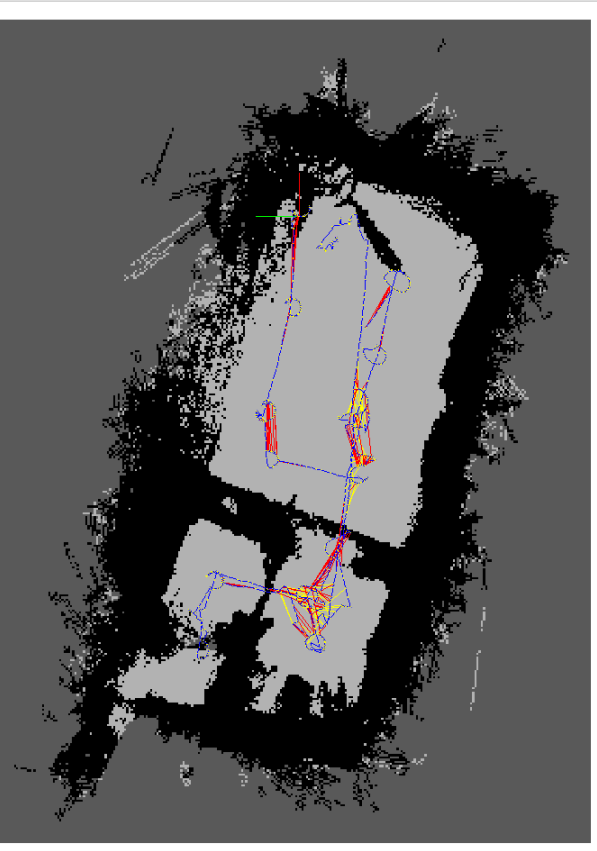
\includegraphics[height=6cm]{Images/mapping graph.png}
    \caption{Mapping Graph}
    \label{fig:mapping_graph}
\end{figure}

\subsubsection{SLAM Limitations and Hybrid Approach Development}

Initial testing of pure RTABMap implementation revealed critical limitations that motivated the development of a hybrid sensor fusion approach. Extended operation testing documented position drift accumulation reaching up to 1.2 meters during 30-minute sessions, with gradual error accumulation particularly pronounced in feature-poor environments or areas with repetitive visual patterns.

Error analysis identified visual odometry drift as the primary contributor, exacerbated by lighting changes, motion blur during movement, and insufficient visual features near walls. Statistical analysis revealed systematic bias in specific movement directions with standard deviations exceeding 40cm for identical positioning commands. Relocalization failures occurred frequently in environments with insufficient distinctive features, requiring manual intervention through robot rotation and often complete database reconstruction when loop closure detection failed catastrophically.

These limitations proved particularly problematic for VR applications requiring precise robot positioning, necessitating the integration of Ultra-Wideband positioning for absolute position reference.

\subsubsection{UWB Positioning System Integration}

The Ultra-Wideband positioning system addresses SLAM drift limitations by providing absolute position reference with centimeter-level accuracy. The UWB integration utilizes the \texttt{uwb\_positioning} package configured through \texttt{uwb.launch.py} with serial communication parameters \texttt{serial\_port\_name: /dev/ttyACM0} and \texttt{serial\_baud\_rate: 115200} for DecaWave hardware interface.

Strategic anchor placement ensures optimal coverage while minimizing Non-Line-of-Sight conditions. The system implements multilateration techniques calculating 3D position from time-of-flight measurements to multiple anchor points.

Position data publishes on \texttt{/UWB/Pos} using \texttt{geometry\_msgs/Pose} format, providing absolute 3D coordinates that serve as the reference for sensor fusion algorithms.

\subsubsection{Hybrid Sensor Fusion Architecture}

The hybrid localization system combines the complementary strengths of visual SLAM and UWB positioning through sophisticated sensor fusion that separates position and orientation estimation. This approach utilizes UWB for absolute position reference while maintaining RTABMap for orientation data, addressing the limitations of each individual system.

\paragraph{Fusion Algorithm Implementation}

The \texttt{\_create\_fused\_pose} method implements core fusion logic prioritizing UWB position data when available, with automatic fallback to RTABMap position estimates during UWB communication failures. Position data undergoes coordinate frame transformation using a configurable 11.5-degree rotation correction through the \texttt{\_apply\_rotation\_to\_pose} method, aligning UWB coordinates with the RTABMap reference frame.

Orientation estimation maintains RTABMap quaternion data as the primary source with validation to detect loss conditions. The system monitors for invalid quaternion values (x=1.0, y=0.0, z=0.0, w=0.0) indicating RTABMap odometry failure and automatically triggers the \texttt{/reset\_odom} service while maintaining position tracking through UWB data.

\paragraph{Orientation Recovery and Fallback Mechanisms}

The system implements sophisticated orientation recovery mechanisms to handle RTABMap orientation loss scenarios that commonly occur in feature-poor environments or during rapid robot movements. Orientation loss detection utilizes specific invalid quaternion values (x=1.0, y=0.0, z=0.0, w=0.0) as failure indicators from RTABMap's visual odometry system.

\paragraph{Movement-Based Orientation Estimation}

Upon detecting orientation loss, the \texttt{\_estimate\_orientation\_from\_movement} method activates a movement-based orientation recovery algorithm that reconstructs robot heading from position trajectory analysis. The algorithm maintains a configurable position history buffer (default 5 positions) storing recent UWB position measurements with temporal validation ensuring minimum 5cm movement thresholds between consecutive measurements to avoid noise-induced false orientation estimates.

The orientation calculation employs vector analysis of the most recent position displacement:
\begin{align}
\Delta x &= x_{current} - x_{previous} \\
\Delta y &= y_{current} - y_{previous} \\
\text{yaw} &= \arctan2(\Delta y, \Delta x)
\end{align}

Movement magnitude validation prevents orientation estimation from small positional noise by requiring displacement magnitude $\sqrt{\Delta x^2 + \Delta y^2} \geq 0.05$ meters. The calculated yaw angle converts to quaternion representation for ROS2 compatibility using standard rotation matrix transformations around the Z-axis:
\begin{align}
q_x &= 0.0 \\
q_y &= 0.0 \\
q_z &= \sin(\text{yaw}/2) \\
q_w &= \cos(\text{yaw}/2)
\end{align}

\paragraph{Multi-Layer Orientation Fallback Strategy}

The orientation selection hierarchy implements three prioritized fallback levels ensuring continuous operation during various failure scenarios. Primary orientation source utilizes live RTABMap quaternion data when valid, providing high-frequency orientation updates with sub-degree accuracy from visual-inertial odometry. Secondary fallback activates movement-based estimation during RTABMap failures, calculating orientation from UWB position displacement vectors with update rates limited by robot movement speed and position measurement frequency.

Tertiary fallback maintains the last valid RTABMap orientation when insufficient movement data exists for estimation, preserving orientation continuity during stationary periods or initialization phases. Ultimate fallback defaults to identity quaternion (0,0,0,1) representing zero rotation when no orientation data is available, ensuring system operation continuity with known heading reference.

\paragraph{Automatic Recovery and Validation}

RTABMap orientation recovery monitoring continuously validates incoming orientation data using the \texttt{\_is\_orientation\_valid} method, detecting transitions from invalid to valid quaternion values indicating successful visual tracking reacquisition. Recovery validation triggers automatic switching from movement-based estimation back to RTABMap orientation data, maintaining position tracking continuity through UWB positioning while restoring full 6-DOF pose estimation capability.

The system implements automatic odometry reset functionality through the \texttt{/reset\_odom} service call upon detecting orientation loss, triggering RTABMap's internal relocalization algorithms while maintaining global position reference through UWB data. Service call validation ensures successful odometry reset confirmation before proceeding with orientation recovery procedures.

Performance monitoring tracks sensor health through comprehensive statistics including UWB position availability percentages, RTABMap orientation validity metrics, movement-based estimation activation frequency, and fusion algorithm performance indicators. Diagnostic logging provides detailed recovery event tracking with timestamp correlation enabling post-analysis of orientation loss patterns and recovery effectiveness.

The multi-layered orientation recovery system ensures robust operation in challenging environments where traditional visual SLAM systems typically fail, maintaining navigation capability during extended visual tracking loss while preserving the precision advantages of hybrid UWB-visual positioning for accurate human detection and interaction positioning described in the following subsection.



\subsection{Human Pose Detection with YOLOv11 and TensorRT Optimization}

Effective human-robot interaction requires real-time human pose detection that can identify body positions, gestures, and spatial relationships in dynamic social environments. The computational demands of deep learning-based pose detection on embedded hardware necessitate careful optimization strategies to achieve real-time performance while maintaining detection accuracy for social robotics applications.

\subsubsection{YOLOv11n-Pose Model Selection and TensorRT Optimization}

The YOLOv11n-pose model provides optimal balance between detection accuracy and computational efficiency for the NVIDIA Orin Nano platform. The nano variant utilizes a streamlined architecture with reduced parameter count, enabling real-time inference while maintaining adequate accuracy for social robot interaction requirements and multi-person detection capabilities within the camera's field of view.

Pre-trained model weights eliminate extensive training requirements by leveraging established pose estimation datasets, providing immediate deployment capability with robust performance across diverse human poses and environmental conditions typical of social robot applications.

\paragraph{Model Format Conversion and Engine Optimization}

The optimization pipeline transforms the original \texttt{yolo11n-pose.pt} PyTorch format through sequential conversions: ONNX intermediate format (\texttt{.onnx}) for cross-platform compatibility, followed by TensorRT engine generation (\texttt{.engine}) for hardware-specific optimization. TensorRT optimization analyzes the YOLOv11n-pose network structure and generates optimized CUDA kernels that maximize GPU utilization through layer fusion, precision calibration, and memory access optimization.

Engine generation includes precision optimization techniques evaluating network sensitivity to reduced precision arithmetic, potentially utilizing INT8 quantization while maintaining FP16 or FP32 precision for critical layers requiring higher numerical accuracy. Memory allocation strategies optimize GPU memory usage patterns to prevent fragmentation and minimize allocation overhead during inference operations.

Performance benchmarks on NVIDIA Jetson Orin Nano demonstrate significant optimization gains: TensorRT FP16 achieves 4.53ms inference time compared to 13.70ms for PyTorch format, representing a 3x performance improvement while maintaining mAP50--95 accuracy of 0.5061 versus 0.5101 for the original model. TensorRT INT8 optimization further reduces inference time to 3.70ms with mAP50--95 of 0.4825, providing optimal performance for real-time applications where slight accuracy reduction is acceptable for substantial speed gains.

\subsubsection{ROS2 Pose Detection Node Architecture}

The \texttt{pose\_detection\_node.py} integrates seamlessly with Tino's ROS2 architecture, managing camera input, TensorRT inference execution, and structured result publication for downstream processing systems.

\paragraph{Camera Integration and Preprocessing}

The node subscribes to Oak-D Pro topics \texttt{/right/image\_rect} for monocular grayscale input and \texttt{/stereo/depth} for corresponding depth information required for 3D coordinate calculation. Image preprocessing includes grayscale to BGR conversion for YOLO compatibility using CPU-based OpenCV operations while maintaining real-time performance through efficient memory management.

The BGR format selection stems from OpenCV's historical design choice, which differs from the conventional RGB ordering used in many computer graphics applications. OpenCV internally represents color images in BGR (Blue-Green-Red) channel order, reflecting its origins in computer vision applications where this ordering provided computational advantages on certain hardware architectures. Since YOLO models are typically trained and optimized using OpenCV preprocessing pipelines, maintaining BGR format throughout the processing chain eliminates unnecessary color channel reordering operations that would introduce computational overhead and potential data copying. The \texttt{cv2.COLOR\_GRAY2BGR} conversion replicates the single grayscale channel across all three BGR channels, creating a pseudo-color image that maintains compatibility with YOLO's three-channel input requirements while preserving the original intensity information.

Synchronization mechanisms maintain temporal alignment between grayscale and depth streams through callback-based processing with \texttt{latest\_image} and \texttt{latest\_depth\_image} synchronization, ensuring corresponding depth information availability for each processed frame.

\paragraph{TensorRT Inference and Result Processing}

TensorRT inference utilizes the pre-converted \texttt{yolo11n-pose.engine} model loaded through \texttt{YOLO(model\_path)} initialization with configurable confidence thresholding (default 0.5) and \texttt{verbose=False} parameter. Post-processing extracts pose keypoints, confidence scores, and bounding box information from \texttt{results[0]} objects, implementing confidence-based filtering and closest person selection based on depth measurements.

Error handling provides comprehensive exception management with detailed logging at configurable levels and graceful degradation during model loading failures or inference errors, maintaining operational continuity through robust try-catch blocks around critical processing sections.

The pose detection results feed directly into the 3D positioning system described in the following subsection, enabling spatial localization of detected human poses.

\subsection{Stereo Depth Integration for 3D Human Positioning}

Accurate spatial awareness requires combining 2D pose detection results with precise depth information to enable 3D human positioning capabilities essential for spatial interaction planning and safety monitoring in social robotics applications.

\subsubsection{Oak-D Pro Depth Processing and Validation}

The Oak-D Pro stereo system generates depth maps through stereo vision algorithms, with depth accuracy depending on stereo baseline, camera calibration quality, and environmental factors including lighting conditions and surface textures.

\paragraph{Robust Depth Extraction}

Depth value extraction implements a median-based approach with a 9x9 pixel window around keypoint locations to obtain robust measurements. The \texttt{get\_depth\_at\_point} function performs outlier filtering by calculating median and standard deviation, filtering values more than 2 standard deviations from the median to ensure reliable depth extraction.

For person detection, the \texttt{get\_median\_depth} function extracts depth from a central bounding box region with configurable padding (25\% by default), providing more stable measurements than single-pixel sampling while avoiding background contamination. Depth validation implements comprehensive quality filtering including zero-value rejection, outlier detection based on statistical analysis, and temporal smoothing over a configurable window size (default 3 frames).

\paragraph{3D Coordinate Transformation}

The \texttt{calculate\_3d\_position} function converts camera-frame coordinates using intrinsic parameters from the \texttt{camera\_info.k} array, extracting focal lengths \texttt{fx}, \texttt{fy} and principal point coordinates \texttt{cx}, \texttt{cy} from the calibration matrix. Automatic unit conversion detects depth values greater than 100 for millimeter to meter conversion, followed by depth calibration correction using configurable \texttt{depth\_scale\_factor} (default 0.575) and \texttt{depth\_offset} parameters derived from empirical calibration.

3D coordinate calculation applies the standard pinhole camera model: \texttt{x\_3d = (x - cx) * z / fx} and \texttt{y\_3d = (y - cy) * z / fy}, where corrected depth \texttt{z = z * depth\_scale\_factor + depth\_offset} accounts for systematic depth measurement biases in the Oak-D Pro stereo system.

\subsubsection{3D Skeleton Generation with Temporal Consistency}

The 3D skeleton generation process combines 2D keypoint detections with corresponding depth values to create complete spatial human pose representations with temporal stability for real-time applications.

\paragraph{Keypoint Depth Association and Validation}

Depth value assignment utilizes 2D keypoint pixel coordinates to extract corresponding depth measurements from the stereo depth map with validation ensuring measurements correspond to human body parts rather than background objects. The \texttt{process\_skeleton} function implements sophisticated temporal smoothing where individual keypoint depths are validated against a reference depth calculated as the median of all valid keypoint depths.

Outlier rejection filters keypoint depths deviating more than the configurable \texttt{depth\_outlier\_threshold} (default 30\%) from the reference, replacing them with temporal median depth from a smoothing window. Missing depth handling addresses invalid keypoint scenarios through reference depth fallback when coordinates are invalid ($x \leq 0$ or $y \leq 0$) or depth extraction fails.

Temporal smoothing maintains a \texttt{skeleton\_depth\_history} list with configurable window size (default 3 frames) storing reference depths for median filtering over time, providing stable depth values that reduce measurement jitter while maintaining responsiveness to actual depth changes.

The resulting 3D skeleton data enables comprehensive real-time tracking capabilities, as detailed in the following subsection describing the complete skeleton tracking implementation.



\subsection{Real-time Skeleton Tracking with COCO Keypoint Framework}

Complete human understanding in social robotics requires comprehensive skeleton tracking that captures body posture, gesture recognition, and movement patterns. The standardized COCO keypoint framework provides a robust foundation for consistent pose representation, enabling reliable gesture analysis and human behavior understanding essential for natural human-robot interaction.

\subsubsection{17-Keypoint COCO Detection Schema}

The implementation utilizes the established COCO pose estimation standard identifying 17 key body joints: nose (0), left eye (1), right eye (2), left ear (3), right ear (4), left shoulder (5), right shoulder (6), left elbow (7), right elbow (8), left wrist (9), right wrist (10), left hip (11), right hip (12), left knee (13), right knee (14), left ankle (15), and right ankle (16).

Joint indexing follows established COCO conventions ensuring compatibility with existing pose analysis tools and datasets, enabling straightforward integration with pose analysis algorithms and facilitating comparison with other human pose detection systems. Keypoint connectivity defines skeletal structure through predefined joint relationships representing human anatomical connections including head structure (nose-eyes-ears), torso connections (shoulders-hips), and limb chains (shoulder-elbow-wrist, hip-knee-ankle) that enable skeletal validation and pose completeness assessment.

\paragraph{Confidence Scoring and Quality Assessment}

Confidence score extraction provides reliability metrics for each detected keypoint, with values ranging from 0.0 (undetected) to 1.0 (high confidence) indicating detection algorithm certainty in keypoint localization accuracy. Quality thresholding implements confidence-based filtering excluding low-confidence detections from downstream processing, with threshold values balancing detection completeness against accuracy requirements typically ranging from 0.3 to 0.7 depending on application requirements and environmental conditions.

Multi-person confidence handling manages confidence scores when multiple humans are detected simultaneously, maintaining separate confidence profiles for each detected person while implementing consistency checks ensuring skeletal coherence within individual pose detections.

\subsubsection{Data Processing Pipeline and Skeleton Organization}

The data processing pipeline transforms raw YOLOv11 output into structured skeleton representations suitable for real-time robot applications through coordinate extraction, normalization, and validation procedures.

\paragraph{Coordinate Processing and Validation}

Raw network output processing extracts keypoint coordinates and confidence scores from YOLOv11 inference results, handling variable-length outputs accommodating different numbers of detected humans while maintaining consistent data structures. Coordinate normalization converts pixel coordinates to standardized coordinate systems enabling consistent processing regardless of camera resolution or field of view variations.

Geometric consistency validation implements anatomical constraints verifying reasonable joint relationships within detected skeletons, including bone length checks, joint angle limitations, and bilateral symmetry assessments that identify and filter implausible pose detections. Temporal consistency analysis compares consecutive pose detections to identify and smooth measurement noise while detecting rapid pose changes indicating genuine human motion.

Completeness assessment evaluates skeleton quality based on the number and distribution of successfully detected keypoints, with assessment criteria including minimum keypoint requirements, critical joint detection (head, torso, limbs), and pose coverage metrics indicating skeleton suitability for specific applications.

\subsubsection{ROS2 Integration and Multi-Modal Data Publishing}

The skeleton tracking system publishes comprehensive pose data through multiple ROS2 topics enabling integration with various robot systems and applications, providing different data formats optimized for specific use cases.

\paragraph{Multi-Topic Publishing Architecture}

The system implements specialized publishers for different data requirements: \texttt{/pose\_detection/image\_raw} for annotated detection images enabling visual debugging, \texttt{/human\_position} for smoothed human position using \texttt{PoseStamped} messages optimized for robot controller integration, \texttt{/human\_skeleton} for 3D skeleton visualization using \texttt{MarkerArray} messages suitable for RViz display, and \texttt{/human\_skeleton\_poses} for programmatic access to joint coordinates using \texttt{PoseArray} messages.

Multi-person handling focuses on closest person selection based on depth measurements, identifying the person with minimum depth value and processing only that individual's skeleton data. This approach reduces computational overhead while ensuring consistent tracking of the most relevant human for interaction applications, with automatic selection providing safety prioritization.

Timestamp synchronization utilizes \texttt{self.get\_clock().now().to\_msg()} for all published messages with consistent \texttt{header.frame\_id} set to the configurable camera frame (default: \texttt{oak\_right\_camera\_optical\_frame}), ensuring temporal alignment across all pose-related data streams.

\paragraph{Robot Controller and VR System Integration}

Robot controller integration subscribes to \texttt{/human\_position} topic for spatial awareness applications where human position data undergoes temporal smoothing through the \texttt{publish\_human\_position} function maintaining a configurable history buffer (default 5 positions) and publishing averaged coordinates to reduce measurement jitter while maintaining responsiveness to human movement.

Pose-based behavior triggers utilize multiple data streams including raw skeleton data from \texttt{/human\_skeleton\_poses} for detailed joint analysis, smoothed position data from \texttt{/human\_position} for proximity detection, and visual markers from \texttt{/human\_skeleton} for debugging and visualization purposes. Safety monitoring implementation prioritizes closest person detection ensuring safety systems focus on the most immediate interaction partner.

VR system integration transmits skeleton data through the dedicated \texttt{vr\_interface\_node.py} described in the software architecture, utilizing the three-port UDP protocol (port 5007 for 208-byte skeleton data at 10Hz) for immersive visualization and interaction analysis. The VR interface node formats skeleton data for Unity applications using the established COCO-format structure with exactly 17 joints, applying default (0,0,0) coordinates for missing joints to maintain data consistency. Data recording capabilities capture complete skeleton tracking sessions for offline analysis through synchronized pose data, camera images, and robot state information published across the multi-topic ROS2 architecture.

The comprehensive skeleton tracking system provides the spatial and temporal human understanding necessary for sophisticated social robot behaviors, with the multi-modal data publishing architecture supporting both real-time robot control and offline analysis requirements for continued system improvement.


